\chapter{Instruction Set Architecture (ISA)}
\section{Cosa è?}
È la struttura attraverso cui tutte le operazioni vengono codificati.

Noi prenderemo d'esempio l'architettura MIPS

\section{Architettura MIPS}
\subsection{Caratteristiche}
\begin{itemize}
    \item Arichitettura di tipo RISC: semplice, uniforme e facile da capire
    \item 32 registri di 32 bit
    \item Permette:
    \begin{itemize}
        \item Manipolazione di dati solo sui registri
        \item Trasferimento di dati tra memoria e registri
        \item Alterazione del flusso di controllo ("Salti" condizionati e non)
    \end{itemize}
\end{itemize}

\section{Formati delle istruzioni}
\begin{itemize}
    \item \textbf{R-Type}: Operazioni tra 2 registri
    \item \textbf{I-Type}: Operazioni immediate tra un registro e un valore "fisso"
    \item \textbf{J-Type}: Operazioni di salto condizionato e non 
\end{itemize}

\section{Rappresentazioni disponibili}
\subsection{Stringa a 32 bit}
\begin{minipage}{0.5\textwidth}
    $$
        00000001000010010101000000100000
    $$
\end{minipage}
\hfil
\begin{minipage}{0.5\textwidth}
    Una semplice stringa di 32 bit consecutivi
\end{minipage}

\subsection{Stringa a 32 bit sezionata}
\begin{minipage}{0.5\textwidth}
    $$
        000000\ 01000\ 01001\ 01010\ 00000\ 100000
    $$
\end{minipage}
\hfil
\begin{minipage}{0.5\textwidth}
    Una semplice stringa di 32 bit consecutivi sezionata con degli spazzi per indicare ogni campo dell'istruzione
\end{minipage}

\subsection{Rappresentazione esadecimale}
\begin{minipage}{0.5\textwidth}
    $$
        0\texttt{x} \ 1 0 9 5 0 2 0
    $$
\end{minipage}
\hfil
\begin{minipage}{0.5\textwidth}
    Una semplice stringa di 32 bit consecutivi sezionata con degli spazzi per indicare ogni campo dell'istruzione
\end{minipage}

\subsection{Formato assembly}
\begin{minipage}{0.5\textwidth}
    \texttt{add \$10, \$8, \$9}
\end{minipage}
\hfil
\begin{minipage}{0.5\textwidth}
    \begin{itemize}
        \item Un formato un pò più comodo:
        \begin{itemize}
            \item codici operativi simbolici
            \item nomi simbolici di registri
            \item nomi simbolici di variabili
        \end{itemize}
        
        \item I registri si trovano a \uline{pagina 24 dell'appendice A}
        \item Gli opcode/funct si trovano a \uline{pagina 50 dell'appendice A}
    \end{itemize}
\end{minipage}

\chapter{ISA R-Type}
\section{Cosa sono?}
Sono tutte quelle istruzioni che coinvolgono l'utilizzo di 3 registri, due registri sorgente e un registro di destinazione al fine di compiere un operazione aritmetico-logica

\section{Struttura}
\subsection{Struttura della stringa a 32 bit}
\begin{center}
    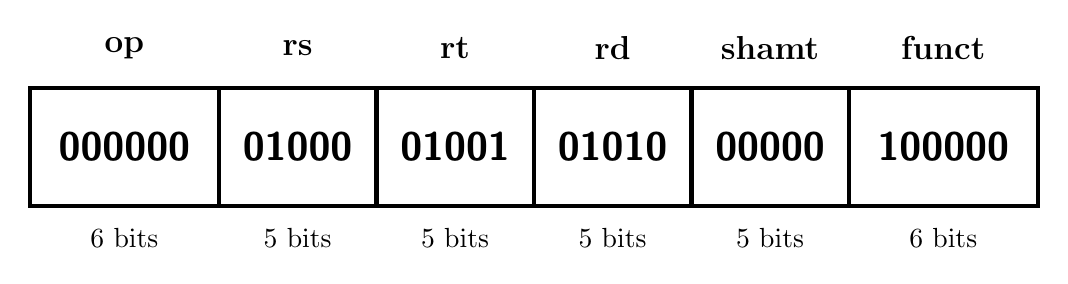
\begin{tikzpicture}[font=\sffamily]
    
        % Stile globale per le linee
        \tikzstyle{every path}=[ultra thick]

        % Disegno il perimetro del registro
        \draw (0,0) rectangle (12.8, 1.5);

        % Linee verticali divisorie (proporzionate a 6-bit e 5-bit)
        \draw (2.4,0) -- (2.4, 1.5);
        \draw (4.4,0) -- (4.4, 1.5);
        \draw (6.4,0) -- (6.4, 1.5);
        \draw (8.4,0) -- (8.4, 1.5);
        \draw (10.4,0) -- (10.4, 1.5);

        % Valori binari interni
        \node at (1.2, 0.75) {\Large \textbf{000000}};
        \node at (3.4, 0.75) {\Large \textbf{01000}};
        \node at (5.4, 0.75) {\Large \textbf{01001}};
        \node at (7.4, 0.75) {\Large \textbf{01010}};
        \node at (9.4, 0.75) {\Large \textbf{00000}};
        \node at (11.6, 0.75) {\Large \textbf{100000}};

        % Nomi dei campi in alto
        \node[font=\large\bfseries] at (1.2, 2) {op};
        \node[font=\large\bfseries] at (3.4, 2) {rs};
        \node[font=\large\bfseries] at (5.4, 2) {rt};
        \node[font=\large\bfseries] at (7.4, 2) {rd};
        \node[font=\large\bfseries] at (9.4, 2) {shamt};
        \node[font=\large\bfseries] at (11.6, 2) {funct};

        % Dimensione in bit in basso
        \node[font=\normalsize] at (1.2, -0.4) {6 bits};
        \node[font=\normalsize] at (3.4, -0.4) {5 bits};
        \node[font=\normalsize] at (5.4, -0.4) {5 bits};
        \node[font=\normalsize] at (7.4, -0.4) {5 bits};
        \node[font=\normalsize] at (9.4, -0.4) {5 bits};
        \node[font=\normalsize] at (11.6, -0.4) {6 bits};

    \end{tikzpicture}
\end{center}

\subsection{Spiegazione dei campi}
\begin{itemize}
    \item \textbf{opcode (6 bit)}: Indica il tipo d'istruzione ISA (R-Type, I-Type, J-Type), per le R-type è sempre 0
    \item \textbf{rs (5 bit)}: Il primo registro sorgente coinvolto nell'operazione
    \item \textbf{rt (5 bit)}: Il secondo registro sorgente coinvolto nell'operazione
    \item \textbf{rd (5 bit)}: Il registro di destinazione della operazione, può essere uno dei 2 registri sorgenti oppure un terzo registro differente
    \item \textbf{shamt (5 bit)}: Indica di quanti bit scorrere il contenuto sorgente durante le operazioni di shift
    \item \textbf{funct (6bit)}: Indica l'operazione da effettuare
\end{itemize}

\chapter{ISA I-Type}
\section{Cosa sono?}
Sono tutte le istruzioni che involgono l'utilizzo di 2 registri e un valore immediato.

Utilizzato per operazioni aritmetico logiche immediate e operazioni di scrittura e lettura in memoria

\section{Struttura}
\subsection{Struttura della stringa a 32 bit}
\begin{center}
    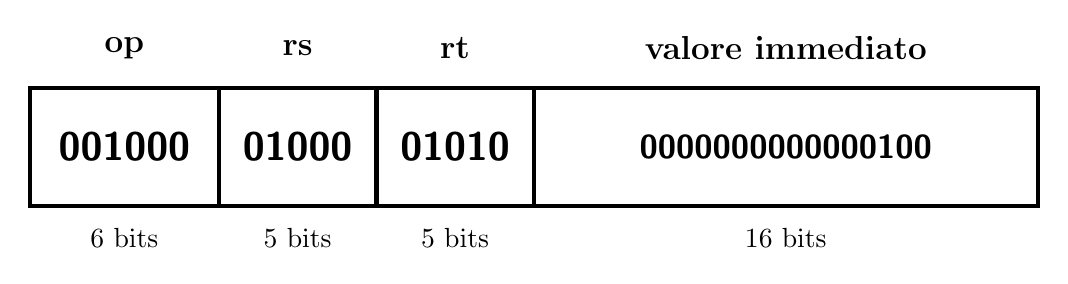
\begin{tikzpicture}[font=\sffamily]
        
        % Stile globale per le linee
        \tikzstyle{every path}=[ultra thick]

        % Disegno il perimetro del registro (lunghezza proporzionale totale 12.8)
        \draw (0,0) rectangle (12.8, 1.5);

        % Linee verticali divisorie (proporzionate a 6-bit, 5-bit, 5-bit, 16-bit)
        \draw (2.4,0) -- (2.4, 1.5);
        \draw (4.4,0) -- (4.4, 1.5);
        \draw (6.4,0) -- (6.4, 1.5);

        % Valori binari interni
        \node at (1.2, 0.75) {\Large \textbf{001000}};
        \node at (3.4, 0.75) {\Large \textbf{01000}};
        \node at (5.4, 0.75) {\Large \textbf{01010}};
        \node at (9.6, 0.75) {\large \textbf{0000000000000100}};

        % Nomi dei campi in alto (sostituiscono i fumetti gialli)
        \node[font=\large\bfseries] at (1.2, 2) {op};
        \node[font=\large\bfseries] at (3.4, 2) {rs};
        \node[font=\large\bfseries] at (5.4, 2) {rt};
        \node[font=\large\bfseries] at (9.6, 2) {valore immediato};

        % Dimensione in bit in basso
        \node[font=\normalsize] at (1.2, -0.4) {6 bits};
        \node[font=\normalsize] at (3.4, -0.4) {5 bits};
        \node[font=\normalsize] at (5.4, -0.4) {5 bits};
        \node[font=\normalsize] at (9.6, -0.4) {16 bits};

    \end{tikzpicture}
\end{center}

\subsection{Spiegazione dei campi}
\begin{itemize}
    \item \textbf{opcode (6 bit)}: Indica quale operazione eseguire
    \item \textbf{rs (5 bit)}: Primo registro (sorgente)
    \item \textbf{rt (5 bit)}: Secondo registro  (destinazione)
    \item \textbf{valore immediato (16 bit)}: Il valore immediato con cui operare
\end{itemize}

\section{Istruzione load word}
\subsection{Struttura stringa a 32 bit}
\begin{center}
    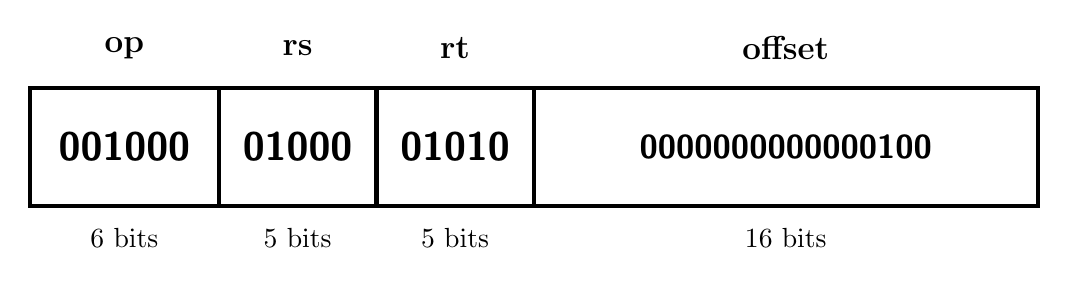
\begin{tikzpicture}[font=\sffamily]
        
        % Stile globale per le linee
        \tikzstyle{every path}=[ultra thick]

        % Disegno il perimetro del registro (lunghezza proporzionale totale 12.8)
        \draw (0,0) rectangle (12.8, 1.5);

        % Linee verticali divisorie (proporzionate a 6-bit, 5-bit, 5-bit, 16-bit)
        \draw (2.4,0) -- (2.4, 1.5);
        \draw (4.4,0) -- (4.4, 1.5);
        \draw (6.4,0) -- (6.4, 1.5);

        % Valori binari interni
        \node at (1.2, 0.75) {\Large \textbf{001000}};
        \node at (3.4, 0.75) {\Large \textbf{01000}};
        \node at (5.4, 0.75) {\Large \textbf{01010}};
        \node at (9.6, 0.75) {\large \textbf{0000000000000100}};

        % Nomi dei campi in alto (sostituiscono i fumetti gialli)
        \node[font=\large\bfseries] at (1.2, 2) {op};
        \node[font=\large\bfseries] at (3.4, 2) {rs};
        \node[font=\large\bfseries] at (5.4, 2) {rt};
        \node[font=\large\bfseries] at (9.6, 2) {offset};

        % Dimensione in bit in basso
        \node[font=\normalsize] at (1.2, -0.4) {6 bits};
        \node[font=\normalsize] at (3.4, -0.4) {5 bits};
        \node[font=\normalsize] at (5.4, -0.4) {5 bits};
        \node[font=\normalsize] at (9.6, -0.4) {16 bits};

    \end{tikzpicture}
\end{center}

\subsection{Spiegazione dei campi}